\documentclass[12pt]{report}

%% ============================================================
%% PACKAGES
%% ============================================================
\usepackage[top=0.75in, bottom=0.5in, left=1.25in, right=1in, headheight=15pt, headsep=16pt]{geometry}
\usepackage{setspace}
\usepackage{graphicx}
\usepackage{amsmath}
\usepackage{amssymb}
\usepackage{hyperref}
\usepackage{caption}
\usepackage{subcaption}
\usepackage{fancyhdr}
\usepackage{titlesec}
\usepackage{listings}
\usepackage{xcolor}
\usepackage{booktabs}
\usepackage{float}
\usepackage{emptypage}   % suppress headers on blank pages
\usepackage{needspace}   % prevent orphaned chapter headings in TOC

%% ============================================================
%% KEEP TOC CHAPTER ENTRIES WITH THEIR SECTIONS
%% ============================================================
\makeatletter
\let\orig@l@chapter\l@chapter
\renewcommand{\l@chapter}[2]{%
    \needspace{8\baselineskip}%
    \orig@l@chapter{#1}{#2}%
}
\makeatother

%% ============================================================
%% SPACING & TYPOGRAPHY
%% ============================================================
\onehalfspacing
\setlength{\parskip}{6pt}

%% ============================================================
%% PAGE BREAK QUALITY
%% ============================================================
\raggedbottom                 % don't stretch pages to fill — let them end naturally
\widowpenalty=9999            % strongly discourage widows (lone last line at top of page)
\clubpenalty=9999             % strongly discourage orphans (lone first line at bottom)
\usepackage{etoolbox}
\preto{\section}{\needspace{5\baselineskip}}  % never start a section near the bottom of a page

%% ============================================================
%% HYPERREF
%% ============================================================
\hypersetup{
    colorlinks = true,
    linkcolor  = black,
    citecolor  = black,
    urlcolor   = blue,
    pdftitle   = {SLAM From Scratch},
    pdfauthor  = {Mario Pardo},
}

%% ============================================================
%% CODE LISTINGS
%% ============================================================
\lstset{
    basicstyle   = \small\ttfamily,
    breaklines   = true,
    frame        = single,
    captionpos   = b,
    numbers      = left,
    numberstyle  = \tiny\color{gray},
    tabsize      = 4,
}

%% ============================================================
%% HEADERS / FOOTERS
%% ============================================================
\pagestyle{fancy}
\fancyhf{}
\renewcommand{\headrulewidth}{0.4pt}
\fancyhead[L]{\small\leftmark}
\fancyhead[R]{\small\thepage}
\fancypagestyle{plain}{%   used on chapter-opening pages
    \fancyhf{}
    \renewcommand{\headrulewidth}{0pt}
    \fancyfoot[C]{\thepage}
}

%% ============================================================
%% CHAPTER TITLE FORMAT
%% ============================================================
\titleformat{\chapter}[block]
    {\normalfont\LARGE\bfseries}
    {\thechapter.}{0.8em}{}
\titlespacing*{\chapter}{0pt}{24pt}{16pt}

%% ============================================================
%% BEGIN DOCUMENT
%% ============================================================
\begin{document}

% ============================================================
%  TITLE PAGE
% ============================================================
\begin{titlepage}
    \centering
    \vspace*{1.5cm}

    {\LARGE \textbf{Carleton University}\\[0.4cm]}
    {\large School of Computer Science\\[0.3cm]}
    {\large COMP 4905 --- Honours Project\\[2.5cm]}

    \rule{\textwidth}{1.5pt}\\[0.6cm]
    {\Huge \textbf{SLAM From Scratch}}\\[0.4cm]
    \rule{\textwidth}{1.5pt}\\[2.5cm]

    \begin{minipage}{0.45\textwidth}
        \centering
        {\large \textbf{Submitted by:}\\[0.3cm]}
        {\large Mario Pardo}
    \end{minipage}
    \hfill
    \begin{minipage}{0.45\textwidth}
        \centering
        {\large \textbf{Supervisor:}\\[0.3cm]}
        {\large Mark Lanthier}
    \end{minipage}

    \vfill
    {\large April 2026}
\end{titlepage}

% ============================================================
%  FRONT MATTER  (Roman numerals)
% ============================================================
\pagenumbering{roman}
\setcounter{page}{1}

% ---- Abstract -----------------------------------------------
\chapter*{Abstract}

Humans are able to navigate and understand new environments quickly and intuitively,
combining sensory inputs with spatial memory to create an understanding of their environment
and their location within it.
Replicating this in machines is a complicated task encompassing various areas of research and
is a key challenge in developing autonomous robots and vehicles.
Simultaneous Localization and Mapping (SLAM) is a class of algorithms dedicated to just this task,
allowing systems to understand the environment in which they operate and where they are within
it --- especially critical in scenarios where external positioning sources, such as GPS, are unavailable.

This project presents a C++ implementation of a Graph-Based SLAM system developed from first
principles.
The resulting system demonstrates reliable convergence in pose-graph optimization, validating
that a ground-up implementation can manage the underlying mathematical complexity and
high-performance requirements of modern robotics.

\newpage

% ---- Acknowledgments ----------------------------------------
\chapter*{Acknowledgments}

% TODO: complete acknowledgments before submission.
\vspace{4cm}
\noindent\textit{Acknowledgments to be completed.}

\newpage

% ---- Table of Contents --------------------------------------
{\pagestyle{plain}\tableofcontents}
\newpage

% ---- List of Figures ----------------------------------------
\listoffigures
\newpage

% ---- List of Tables -----------------------------------------
\listoftables
\newpage

% ============================================================
%  MAIN BODY  (Arabic numerals, starting from 1)
% ============================================================
\pagenumbering{arabic}
\setcounter{page}{1}

% ============================================================
\chapter{Introduction}
% ============================================================

Robotic systems sense the world and themselves through a variety of sensors, such as wheel encoders,
gyroscopes, and lidar sensors.
The two former are combined to create \textit{odometry} data, estimating the change in position and
orientation (pose), while the latter uses laser reflections to sense the geometry of the world at a
distance.
In real-world settings, odometry data carries noise from sensor readings and misalignments between
these readings and the motion they imply --- for example, wheels slipping over bumps.
This causes \textit{drift}: an error in the calculated pose compared to the actual pose.
As pose estimates build on top of one another, this drift accumulates quickly, leading to worsening
estimates and conflicts with incoming sensor data --- ultimately producing catastrophic errors in
localization and mapping.

To illustrate: lidar data might indicate a wall 3~m directly ahead, but the pose estimate says the
robot is at $(3\text{ m},\; 1\text{ m})$ while it is in reality at $(2\text{ m},\; 0\text{ m})$. The
system then believes the wall is at $(6\text{ m},\; 1\text{ m})$ when it is actually at
$(5\text{ m},\; 0\text{ m})$.

A Graph-Based SLAM system constructs a graph of poses and movements, and when it detects a
\textit{loop closure} --- a location previously visited --- it uses this new observation to update all
previous pose estimates, ``snapping'' both trajectory and map into a corrected version.

The intention of this project was to open this algorithmic black box and gain rigorous experience
studying, understanding, implementing, debugging, and testing a complex system from first principles.
Developing a SLAM algorithm tested knowledge in mathematics --- specifically linear algebra and
statistics --- and its application to a complex, multi-step, real-world system written in
high-performance C++.

% ============================================================
\chapter{System Architecture}
% ============================================================

A SLAM system starts with sensor inputs and, over time, accumulates information to locate itself and
map its surroundings.
It is composed of a chain of subsystems of varying complexity, each depending on the step before it
to produce meaningful results.

The system can be broken down into 4 main stages:
\begin{enumerate}
    \item \textbf{Sensor Integration}: Collect sensor data and process into usable odometry data and point clouds
    \item \textbf{Transformation Estimation:} Iterative Closest Point (ICP) to estimate robot motion
and map surrounding environment
    \item \textbf{Pose Graph Construction}: Keep track of trajectory and mapping data through the construction of a Pose Graph
    \item \textbf{Loop Closures and Pose Graph Optimization}: If robot has recognized a familiar pose, try to correct error in pose graph
\end{enumerate}

\begin{figure}[H]
    \centering
    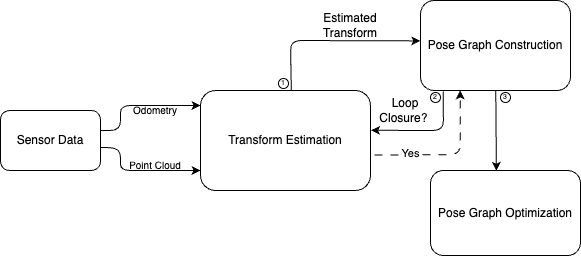
\includegraphics[width=0.72\textwidth]{../images/PG-SLAM_Architecture.png}
    \caption{Visualization of a the data flow and main components of the Pose Graph SLAM System.}
    \label{fig:loop_closure}
\end{figure}

\newpage

\section{Technology Stack}

\textbf{C++ --- Core Algorithm.}
C++ continues to be the language of choice for high-performance code.
Writing the backend in C++ provided an excellent opportunity to make use of its powerful features and
meet the intense performance requirements of robotics software.
Key libraries used:
\begin{itemize}
    \item \textbf{Eigen} --- linear algebra.
    \item \textbf{GTSAM} --- pose graph optimization.
\end{itemize}

\textbf{Webots --- Robotics Simulation.}
Webots is a simple yet powerful open-source robotics simulation platform.
It provides ready-made sandboxes and robot models, such as the TurtleBot Burger 3 used in this
project, with the necessary setup for motion and sensor usage.
Using these ready-made tools allowed focus on the core SLAM implementation and allows for easy
scaling of the project.

\textbf{Python --- Visualization and Communication.}
Python was used on both sides of visualization: interfacing with Webots for robot simulation, and on
the backend for visualizing trajectories, occupancy grids, and system outputs.
It was selected for its ease of use and wide library support.

\textbf{ZeroMQ --- Communication Protocol.}
ZeroMQ was selected for communication between the front end, backend, and visualization tools.
It implements the Publish/Subscribe architecture, which is well suited to a use case where systems
must communicate consistently in both directions without requiring full synchronization.
The name reflects its need for no broker or central server, making it resilient to any single endpoint
failing, and it is straightforward to implement from both C++ and Python.

% ============================================================
\chapter{World Setup and Sensor Integration}
% ============================================================

Various sensors in the robot acquire data at each timestep.
This project makes use of:
\begin{itemize}
    \item \textbf{Wheel encoders} --- measure the rotation of each wheel, processed into odometry data
          that estimates the robot's displacement.
    \item \textbf{Lidar} --- a $360^\circ$ scan of the environment using laser light; the reflection of
          each projected beam records the distance to the nearest surface at a given angle.
\end{itemize}

This data is gathered in Webots and the raw values are forwarded to the C++ backend for processing.

\section{Arena and Robot Setup}

The first step was to set up the testing arena and robot.
A simple square arena was created that is easy to interpret in visualization tools while containing
sufficient detail and landmarks for ICP (Chapter~\ref{chap:icp}) to work with.
The premade TurtleBot Burger 3 was selected, already equipped with all necessary sensors.
A simple differential drive controller was created and tested to confirm reliable movement.

\section{Odometry}

Using the known wheel diameter and wheelbase width, the robot's trajectory is calculated from wheel
sensor data.

\textbf{Noise.}
In a real-world setting, wheel sensors are not perfect.
They can record movement that does not result in actual robot displacement --- such as wheel slip on
wet terrain --- or introduce sensor measurement noise.
Modelling this noise is important, as correcting for it is a core responsibility of the SLAM system.

Odometry provides the first reference point for the SLAM algorithm.
The robot's position was first estimated using odometry alone as a crucial validation step, confirming
that the trajectory can be accurately calculated before introducing additional components.

\section{Point Cloud}

Using simple trigonometry, for each beam from the lidar sensor the landing point --- and therefore
the location of the nearest surface --- can be calculated from the robot's frame of reference.

\textbf{World Frame Projection.}
With the estimated current robot pose, the point cloud is projected into a static world frame,
providing an estimate of where surfaces lie on the map.
An initial visualization tool was implemented to display the robot's trajectory alongside the surfaces
currently observed.
The tool was subsequently upgraded (indicated visually by a dark background) to maintain a history of
all previously observed surfaces, yielding a persistent map of the environment.

\section{Webots Lidar Noise During Rotation}
\label{sec:webots_bug}

Even after introducing rotation gating for localization (described in
Section~\ref{sec:icp_rotation}), significant map smear persisted.
After considerable troubleshooting, the source was identified as a Webots simulator issue: while
the robot is rotating, the lidar scan twitches back and forth and only snaps back into place once
rotation finishes, producing very noisy and incorrect lidar data during the rotation.
The fix was to discard all lidar data collected while the robot is rotating, using only readings when the 
robot is undergoing no rotation, where lidar readings are accurate

\begin{figure}[H]
    \centering
    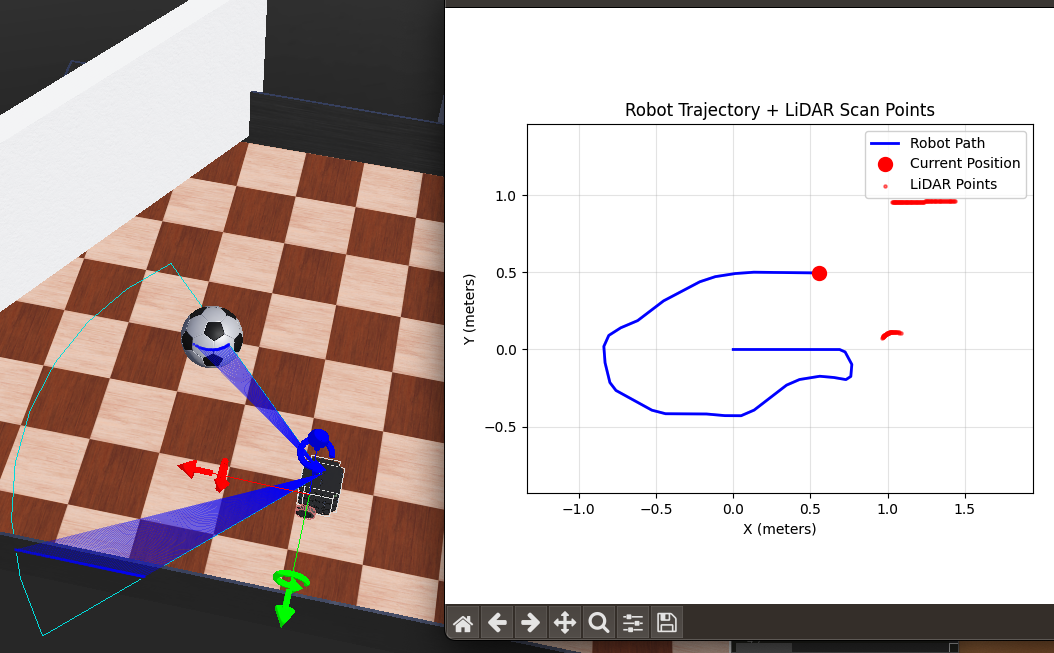
\includegraphics[width=0.72\textwidth]{../images/VisualizeLidarAndTrajTest.png}
    \caption{Initial visualizations showing working trajectory estimation using odometry, and 
    lidar point cloud in robot frame}
    \label{fig:first_traj_lidar_viz}
\end{figure}

% ============================================================
\chapter{Occupancy Grid}
% ============================================================

To accomplish the mapping portion of SLAM, an occupancy grid represents the map by storing the
likelihood that each cell is occupied, encoded using log-odds:

\begin{equation}
    \ell(m_k) = \log \frac{P(m_k \mid z_{1:t},\; x_{1:t})}{1 - P(m_k \mid z_{1:t},\; x_{1:t})}
\end{equation}

where $m_k$ is the $k$-th cell, $z_{1:t}$ is the history of sensor readings, and $x_{1:t}$ is the
history of poses.
As the robot receives lidar returns, the likelihood of occupied cells along each beam is increased,
and cells along the free path are decreased.

The occupancy grid is only updated on new keyframes (Chapter 6) to ensure readings come from stable
and trusted data. 

% ============================================================
\chapter{ICP: Scan Matching}
\label{chap:icp}
% ============================================================

Iterative Closest Point (ICP) is one of the most crucial components of the SLAM system.
It takes two point cloud readings --- a previous scan and a current scan --- and estimates how the
robot has moved between them.

The algorithm, at a high level, proceeds as follows: \newline

\noindent\textbf{alignPointClouds}$\left(\texttt{sourcePointCloud},\; \texttt{targetPointCloud},\; \texttt{odometryInitialGuess}\right)$
\begin{enumerate}
    \item Transform the source point cloud by the initial guess provided by odometry.
    \item \textbf{Find correspondences}: identify which points in the source and target clouds
          represent the same surface.
    \item Using these correspondence pairs, \textbf{estimate the transformation} between the two
          clouds.
    \item Update the current estimate with the refined transformation.
    \item If the change in error falls below a threshold, ICP has \textbf{converged}.
\end{enumerate}

\section{Correspondence Matching}

The most simple method of correspondence matching was used. 
The logic goes as follows for each point in the source cloud, the closest
point in the target cloud is found and the pair is considered a correspondence.

A key hyperparameter is \texttt{max\_distance}, the maximum distance at which two points can be
paired.
This is a trade-off between precision (smaller distance yields more accurate transformations) and
generality (too small a distance results in too few matches).


\section{Estimating the Transform}

Given the set of correspondences, the transformation is estimated using the Singular Value Decomposition (SVD) method.

Let $\mu_s$ and $\mu_t$ denote the centroids of the source and target point sets respectively. Let $W = \sum_i (p_i - \mu_s)(q_i - \mu_t)^\top$ be their cross-covariance. Taking their outer product tells us how each pair of axes from each group correlates. 

The SVD of $W$ is given by $W = U D V^\top$. We can interpret $V$ as the directions coming \textbf{into} the transformation, $U$ as the transformed \textbf{output} direction vectors for those same inputted directions, and $D$ as the scaling for each direction. 

From this, we get the optimal rotation:
\begin{equation}
    R = V U^\top
\end{equation}

And then to get the full transformation, we find the translation from the rotated source centroid to the output centroid:
\begin{equation}
    t = \mu_t - R\,\mu_s
\end{equation}

Since a straightforward analytical solution is known, implementation was a matter of correctly
converting these equations into code, verified by unit tests.

\section{Convergence}

The error between successive transformation estimates is computed.
If it falls below a threshold, ICP is considered converged.
This required hyperparameter tuning: errors were printed across many runs, the best 10\% were
identified, and the threshold was iteratively narrowed to one that gave consistent yet precise
convergences.

\section{Handling Rotation}
\label{sec:icp_rotation}

Large rotations cause point clouds to change drastically from little robot movement, so ICP
inherently struggles to find good transformations during rapid rotation.
To address this, \textit{gating} was introduced: if the robot's angular velocity exceeds a threshold,
the odometry-estimated transformation is used instead of running ICP.
This is a simple and effective fix, though a production system would use more sophisticated sensor
fusion such as an Extended Kalman Filter to intelligently weight sensor sources when any one cannot be
fully relied upon.

Expanding the lidar field of view from $90^\circ$ to $360^\circ$ was a major breakthrough for ICP
accuracy and consistency.
With a $90^\circ$ FOV, even small rotations shift a large fraction of the visible point cloud,
making correspondence matching difficult.
With a full $360^\circ$ view, surfaces all around the robot remain visible throughout rotation,
providing ICP with stable correspondences.

\section{ICP 180-Degree Inversion Bug}

Early in testing, ICP produced transformations at $180^\circ$ from the actual movement.
The initial patch manually rotated the output by $180^\circ$, which worked but was clearly a symptom
of a deeper issue.

The root cause was a source/target mismatch.
Consider a robot at $(0,0)$ with a wall at $(0,2)$.
From the robot's frame, the wall is 2~m ahead.
After the robot moves forward 1~m to $(0,1)$, the wall appears 1~m ahead: from the robot's frame the
wall has moved by $(0,-1)$.
This is geometrically correct from the robot's point of view, but produces an inverted transformation.

To correct this, the source and target must be swapped.
If the source point is at relative position $(0,1)$ and the target at $(0,2)$, the transformation
found is $(0,+1)$, which correctly describes the robot's forward motion.


\begin{figure}[H]
    \centering
    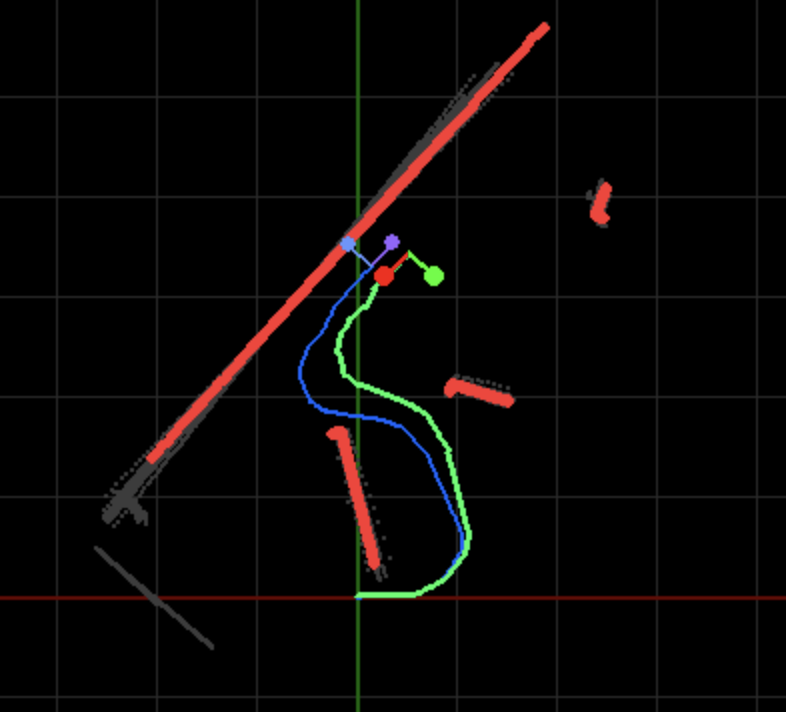
\includegraphics[width=0.3\textwidth]{../images/WorkingICP.png}
    \caption{Initial working ICP implementation, still dealing with mentioned rotation smear}
    \label{fig:first_traj_lidar_viz}
\end{figure}

% ============================================================
\chapter{Pose Graph Construction}
% ============================================================

The pose graph is the record of where the robot has been and how the world has appeared at each
timestep.

\textbf{Graph Nodes} contain:
\begin{itemize}
    \item \textbf{Pose} --- estimated position $(x, y)$ and heading angle $\theta$.
    \item \textbf{Point cloud} --- how the world appeared at this pose.
    \item \textbf{ID and Timestamp} --- for identification and ordering.
\end{itemize}


\begin{figure}[H]
    \centering
    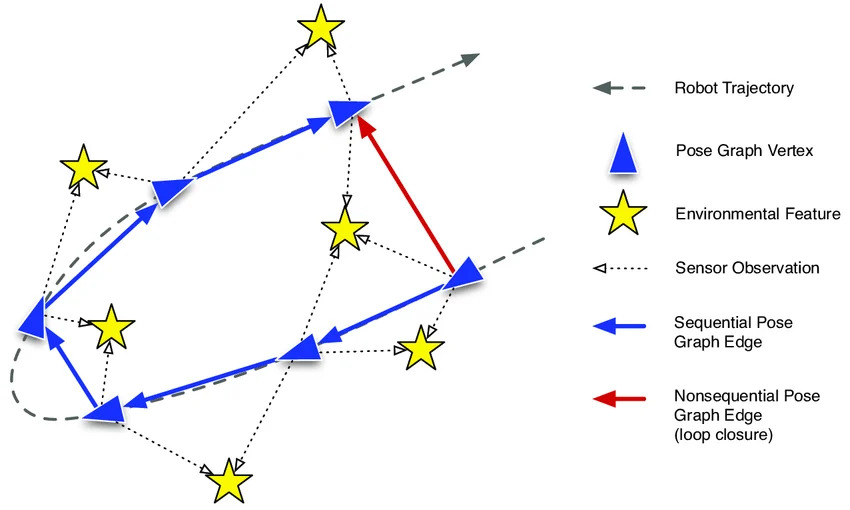
\includegraphics[width=0.6\textwidth]{../images/PoseGraphDiagram.jpg}
    \caption{Diagram of Pose Graph and it's meaning}
    \label{fig:pose_graph}
\end{figure}


\textbf{Edges} represent the robot movement between nodes as calculated by ICP

Nodes (keyframes) are added only once the robot has moved a minimum distance $d$ or rotated a minimum
angle $\delta\theta$, tuned through trial and error.
This is a trade-off: too many nodes overwhelm the optimizer; too few forces ICP to find
transformations across large gaps.
For a square world nearly 2~m diagonally across, a keyframe step of 15~cm was large enough not to
overwhelm the optimizer while small enough for ICP to find accurate transformations.

The visualization tool was updated to display graph nodes and their ICP-estimated edges.

% ============================================================
\chapter{Loop Closure Detection}
% ============================================================

As the robot traverses the world and adds keyframes, the current position is compared with old graph
nodes to detect whether a previously visited location has been returned to.
An exact match is not required; being within a sufficient proximity is enough.
If a candidate is found, ICP is run against the old node's point cloud to confirm the loop closure
and obtain a precise relative pose estimate.
A special \textit{loop closure edge} is then added between the current node and the matched old node.

\begin{figure}[H]
    \centering
    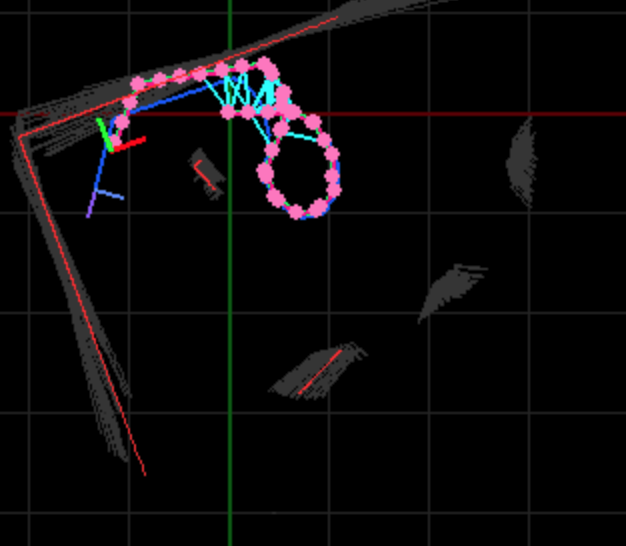
\includegraphics[width=0.5\textwidth]{../../Pictures/ProgressPics/LoopClosure}
    \caption{Visualization of a detected loop closures (cyan) and the resulting graph edge connecting the
             current pose to a previously visited node.}
    \label{fig:loop_closure}
\end{figure}

If no good match is found, or ICP does not converge on a consistent transformation, the robot
continues accumulating keyframes as normal.

While loop closures reuse much of the ICP infrastructure, they are a crucial step: they determine
when and how the graph is optimized, and therefore when accumulated error is corrected.

Hyperparameter tuning was required, notably for correspondence distance and error epsilon.
The goal is accurate loop closure edges that are also general enough to reliably trigger when
revisiting a location.
Too selective, and loop closures never trigger; too permissive, and false closures corrupt the graph.

\section{Performance Tuning}

Loop closure detection requires running ICP repeatedly --- a computationally expensive process ---
so the set of candidate nodes is filtered aggressively before ICP is invoked:

\begin{itemize}
    \item \textbf{Recency filter.}
          Useful loop closures only involve nodes from well before the current position.
          Only nodes at least $N = 10$ keyframes back are considered.

    \item \textbf{Proximity filter.}
          A loop closure requires physical proximity.
          The 6 closest candidate nodes by Euclidean distance are retained before running ICP.

    \item \textbf{Temporal gating.}
          Once a loop closure has been added, subsequent closures in the same vicinity provide
          diminishing benefit and can challenge the optimizer.
          Loop closure attempts are therefore gated to a minimum of 3 keyframes after the last
          successful closure, providing significant computational savings without limiting
          system effectiveness.
\end{itemize}

% ============================================================
\chapter{Pose Graph Optimization}
% ============================================================

With a loop closure edge added, the graph forms a full loop and is ready to be optimized.
Optimization finds the arrangement of node poses that minimizes the total error across all edges.
This step is what "snaps" the map in place, through the reduction of acculumated drift

\section{Problem Formulation}

Let $\mathbf{x} = \{x_1, x_2, \ldots, x_n\}$ denote the state: the set of node poses.
Let $\hat{z}_{ij}$ denote the \textit{measured relative pose} between nodes $i$ and $j$, as
estimated by ICP.
Let $z_{ij}(\mathbf{x})$ denote the \textit{predicted relative pose}, computed from the difference
in stored node coordinates.

The error for edge $(i,j)$ is:
\begin{equation}
    e_{ij}(\mathbf{x}) = z_{ij}(\mathbf{x}) - \hat{z}_{ij}
    \label{eq:error}
\end{equation}

Each edge carries an information matrix $\Omega_{ij}$, representing confidence in the measurement
(derived from how much the ICP result differed from the odometry prediction).
The weighted squared error per edge is:
\begin{equation}
    \varepsilon_{ij}(\mathbf{x})
        = e_{ij}(\mathbf{x})^\top\, \Omega_{ij}\, e_{ij}(\mathbf{x})
\end{equation}

Thus, to minimize error, the optimization goal is:
\begin{equation}
    \mathbf{x}^* = \arg\min_{\mathbf{x}}\;
        \sum_{(i,j) \in \mathcal{E}} e_{ij}(\mathbf{x})^\top\, \Omega_{ij}\, e_{ij}(\mathbf{x})
    \label{eq:opt_goal}
\end{equation}

\section{Solving via Iterative Local Linearization}

This nonlinear least-squares problem is solved using iterative local linearization, upon which the
Levenberg--Marquardt optimizer builds.

\textbf{Step 1 --- Linearize around the current estimate.}
\begin{equation}
    e_{ij}(\mathbf{x} + \Delta\mathbf{x})
        \approx e_{ij}(\mathbf{x}) + J_{ij}\,\Delta\mathbf{x}
\end{equation}
where $J_{ij}$ is the Jacobian of $e_{ij}$ with respect to $\mathbf{x}$.
Linearizing transforms a curved error landscape into a locally flat one that can be solved with
linear algebra.

\textbf{Step 2 --- Expand the squared error in terms of $\Delta\mathbf{x}$.}
\begin{align}
    \varepsilon_{ij}
        &= \bigl(e_{ij} + J_{ij}\Delta\mathbf{x}\bigr)^\top
           \Omega_{ij}
           \bigl(e_{ij} + J_{ij}\Delta\mathbf{x}\bigr) \nonumber \\
        &= \underbrace{e_{ij}^\top \Omega_{ij} e_{ij}}_{C_{ij}}
         + 2\underbrace{e_{ij}^\top \Omega_{ij} J_{ij}}_{b_{ij}^\top}\Delta\mathbf{x}
         + \Delta\mathbf{x}^\top
           \underbrace{J_{ij}^\top \Omega_{ij} J_{ij}}_{H_{ij}}
           \Delta\mathbf{x}
    \label{eq:expand}
\end{align}
where $b_{ij} = J_{ij}^\top\Omega_{ij}\,e_{ij}$ encodes the gradient direction and
$H_{ij} = J_{ij}^\top\Omega_{ij}J_{ij}$ is the Gauss--Newton Hessian approximation.

\textbf{Step 3 --- Differentiate, set to zero, and solve for $\Delta\mathbf{x}$.}
The GTSAM solver handles this step internally, iterating until convergence.

\section{Implementation}

GTSAM is a well-known and well-tested pose graph optimization library.
A \texttt{FactorGraph} was constructed from the existing \texttt{PoseGraph} data structure and
passed to GTSAM's Levenberg--Marquardt optimizer.
The optimized poses were then written back into the graph, and the point clouds of each node were
reprojected at the updated pose coordinates to remove map smear accumulated from drift.

Similar to loop closure, pose graph optimization is computationally heavy.
It is therefore gated to a minimum of 10 keyframes since the last optimization run.

Initial attempts produced unexpected graph translations and, most notably, no improvement to
mapping --- smear was not removed.
This led to a thorough evaluation of the full SLAM pipeline, including implementation of
point-to-plane correspondence matching in ICP and iterative hyperparameter refinement.
The Webots lidar rotation issue (Section~\ref{sec:webots_bug}) was discovered during this
investigation, and resolving it was the key breakthrough that brought the full system together.

% ============================================================
\chapter{Results}
% ============================================================

This project produced a working and reliable SLAM implementation able to localize the trajectory
of the robot and provide an accurate occupancy grid map of its surroundings within the testing
environment.

Creating an entire SLAM system from scratch, without prior experience in the field, is a substantial
undertaking that tested system architecture skills and the ability to design, implement, and debug
complex code with direct real-world applications.

\section{Trajectory Accuracy}

The success of the system is clearly visible in the trajectory results.
ICP demonstrably uses lidar information to calculate trajectories that smooth and correct the errors
introduced by noisy odometry.

In the image below we can see the remarkable accuracy of ICP and our Pose Graph in trajectory mapping.
We have ICP trajectory in green, Odometry trajectory in blue, ground truth trajectory in white. 
As well as Pose Graph nodes in pink with their ground truth transformation in a dark pink. 
We see that ICP in green actually hides the ground truth trajectory, shown in white, only visible at some spots,
which goes to show that the estimated trajectory is virtually identical to the ground truth trajectory.
We see a slight shift between the Pose Graph nodes and ICP, and this is a result of our Pose Graph Optimization.


\begin{figure}[H]
    \centering
    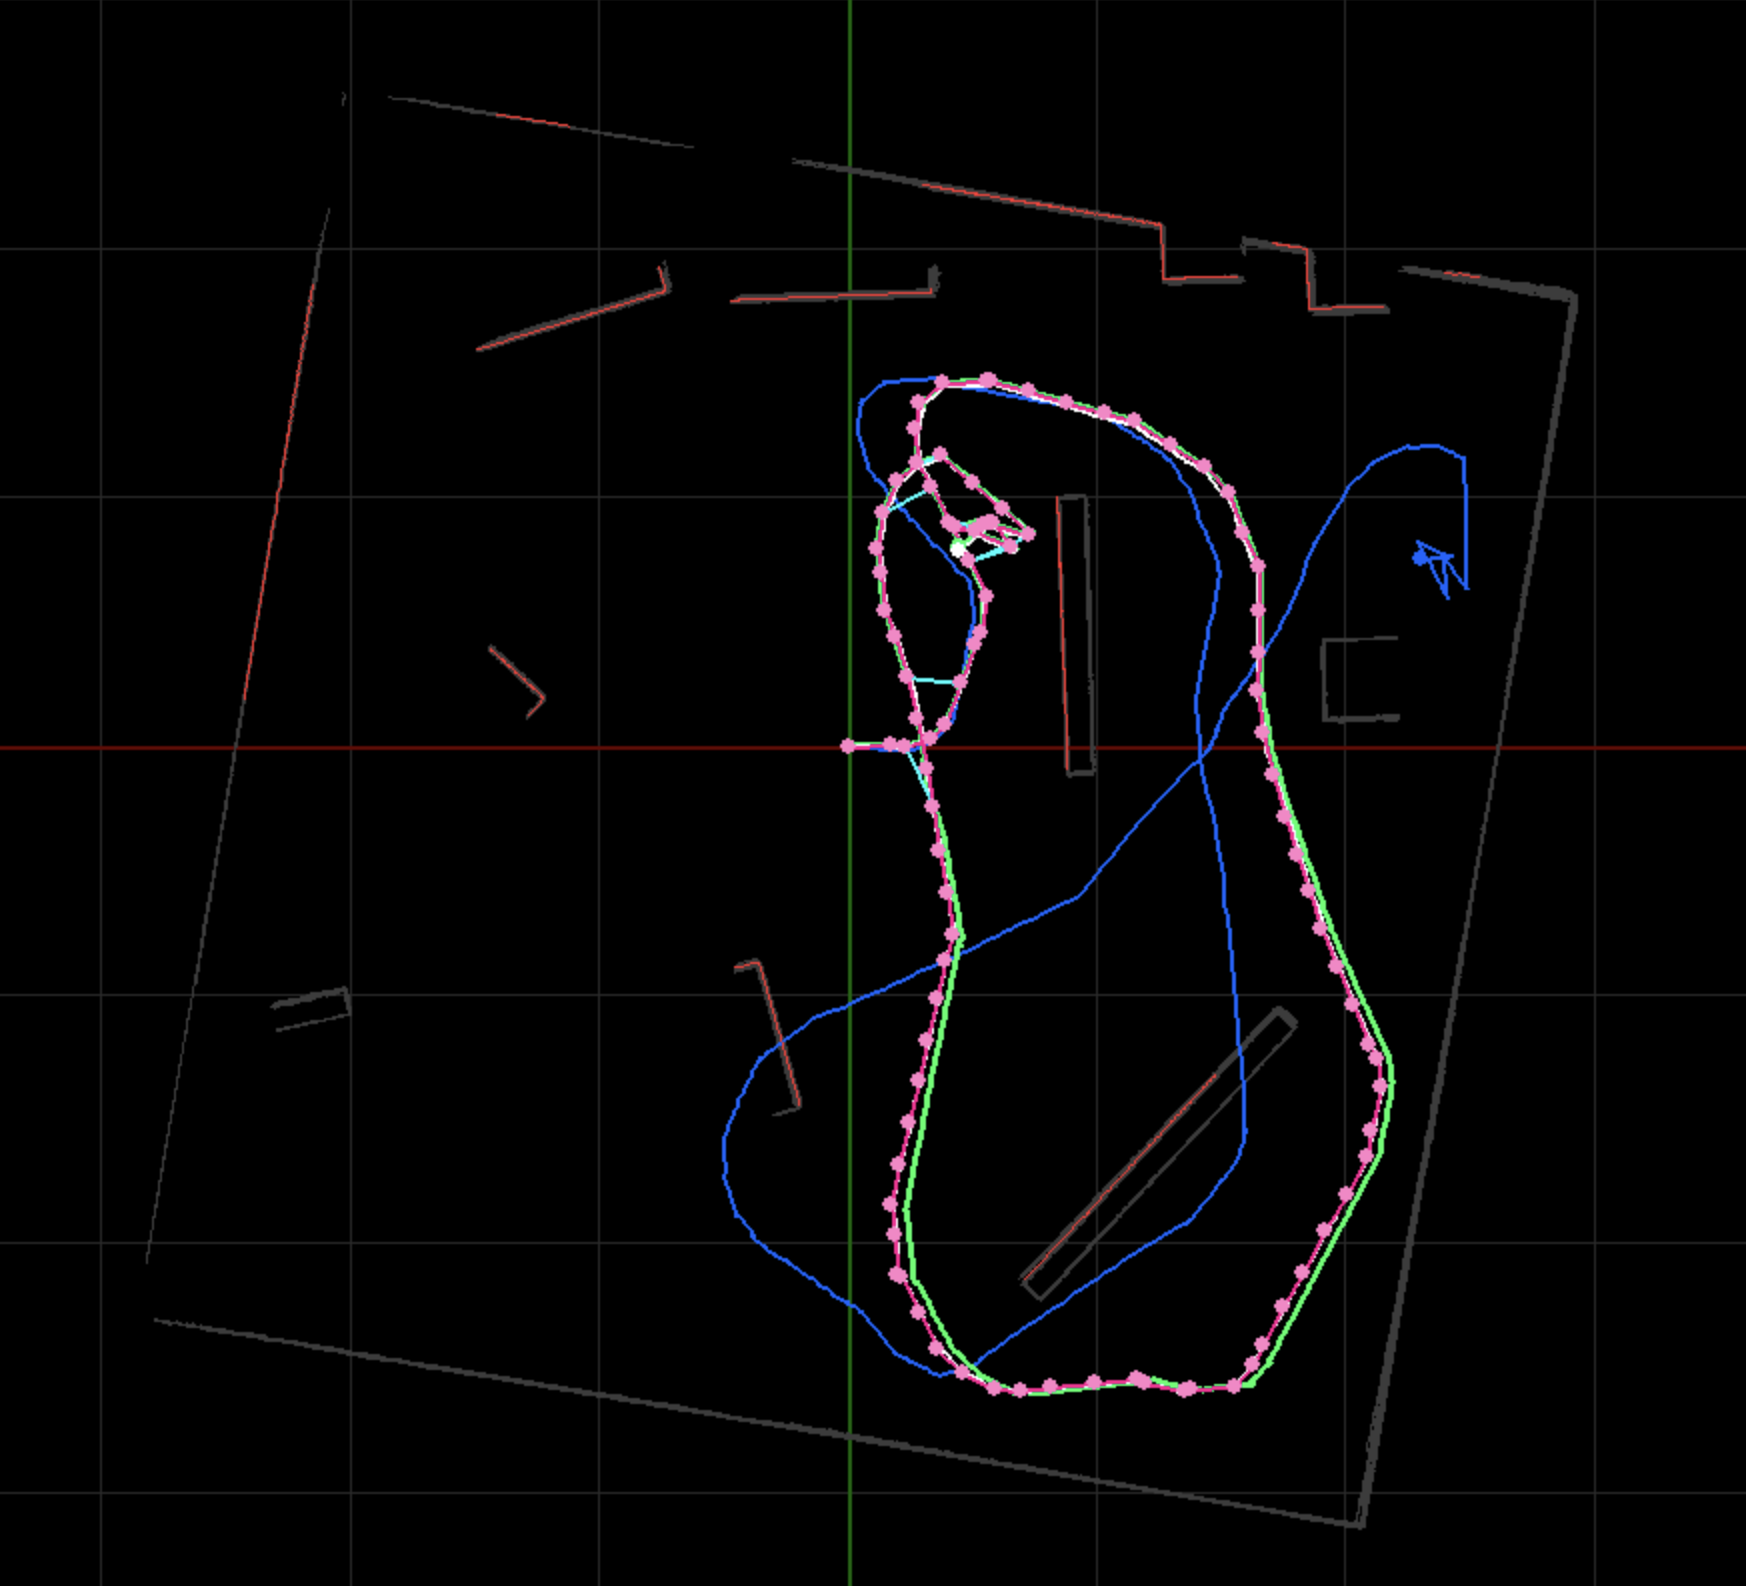
\includegraphics[width=0.4\textwidth]{../images/ICP_vs_Odom_FullMap.png}
    \caption{Final Trajectories and Pose Graph in simulation environment  }
    \label{fig:traj_icp_vs_odom}
\end{figure}

\section{Mapping Accuracy}

The improvement in map quality from using ICP over raw odometry is clearly visible in the image below. 
We see how ICP does not smear like odometry does

\begin{figure}[H]
    \centering
    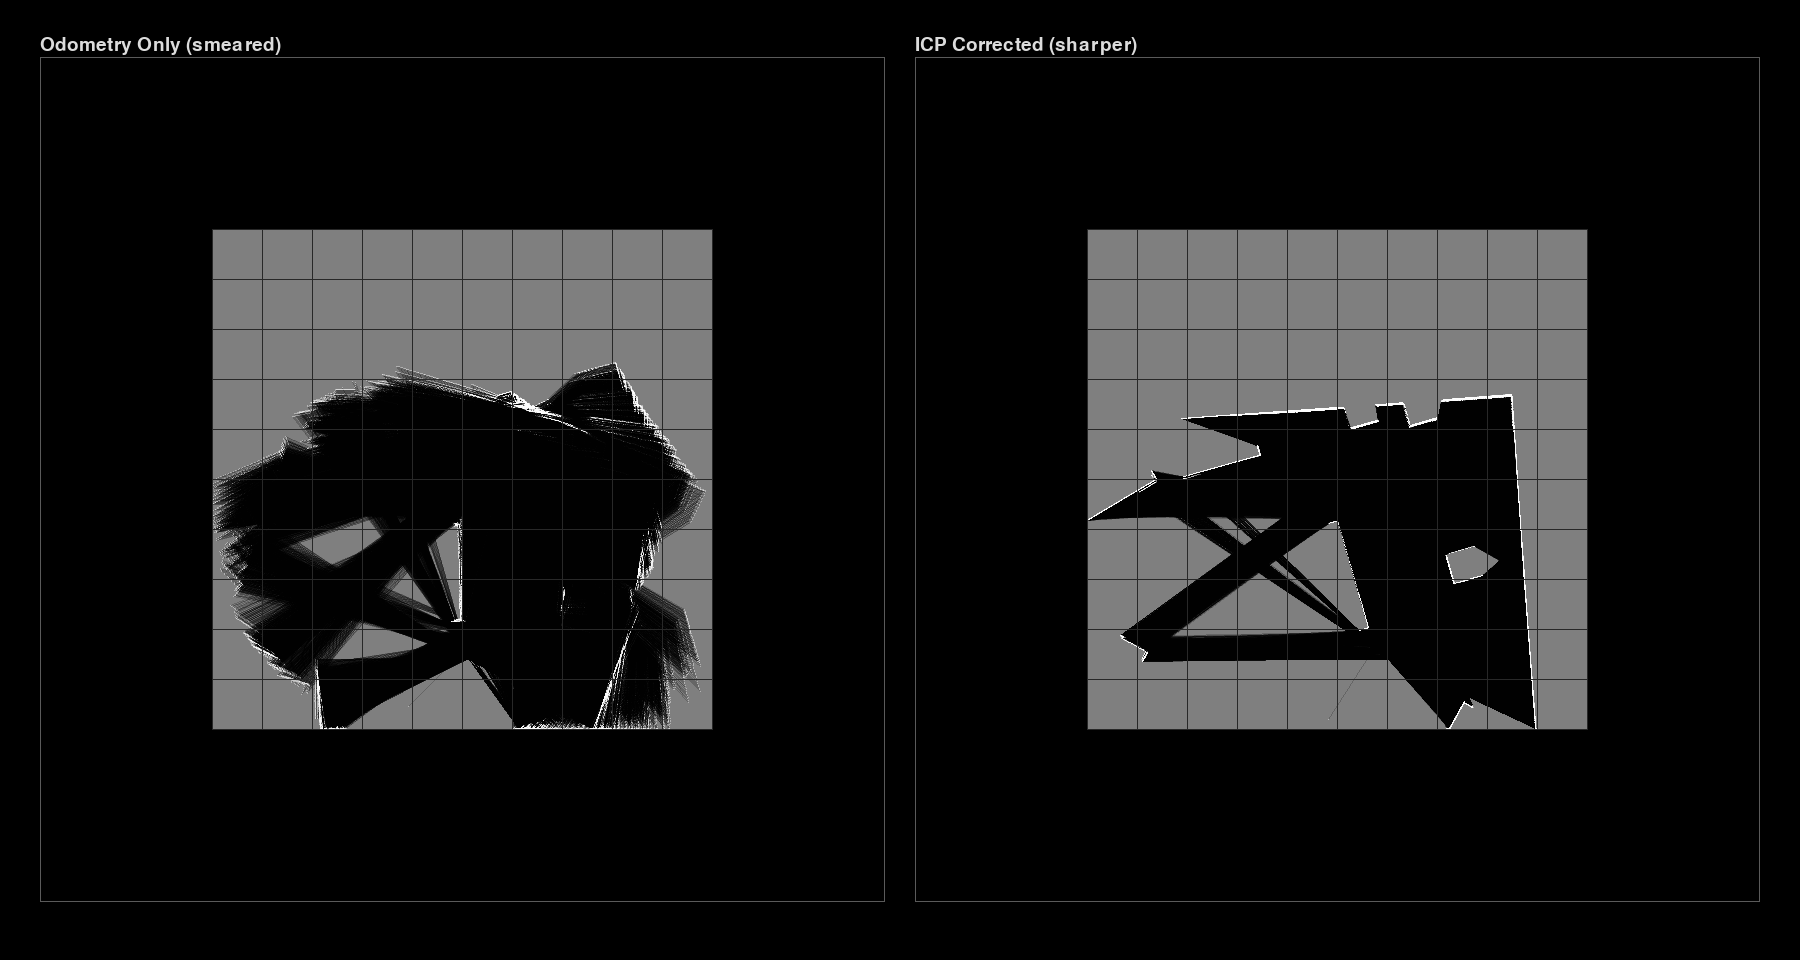
\includegraphics[width=0.5\textwidth]{../images/Odometry_vs_ICP_Mapping_midtraj.png}
    \caption{In progress occupancy grid from Odometry(left) and ICP(right)  }
    \label{fig:traj_icp_vs_odom}
\end{figure}

And when we visualize the final output of our occupancy grid compared to our actual simulation environment, we see
the remarkable success of the SLAM system.

\begin{figure}[H]
    \centering
    \begin{subfigure}[t]{0.32\textwidth}
        \centering
        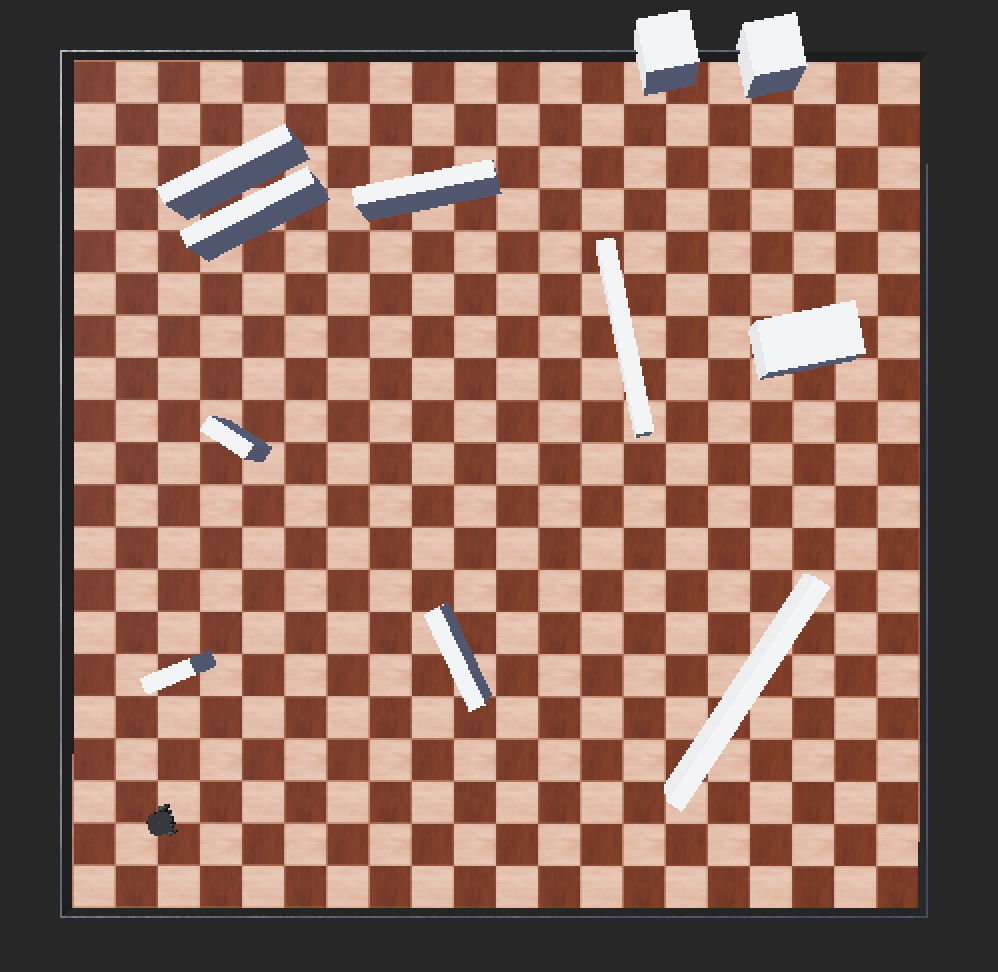
\includegraphics[width=\textwidth]{../images/GroundTruthSimEnv}
        \caption{Simulation environment ground truth.}
        \label{fig:simenv_ground_truth}
    \end{subfigure}
    \hspace{0.3in}
    \begin{subfigure}[t]{0.32\textwidth}
        \centering
        \includegraphics[width=\textwidth]{../images/SimEnv_Output_OccGrid}
        \caption{Output occupancy grid.}
        \label{fig:simenv_occ_grid}
    \end{subfigure}
    \caption{Ground truth vs. SLAM occupancy grid output for the simulation environment.}
    \label{fig:simenv_gt_vs_occgrid}
\end{figure}

\section{Pose Graph Optimization}

Given the small map size ($\approx 2\times 2$~m), insufficient drift accumulates to produce a
visually dramatic graph snap.
The improvement can, however, be quantified through the reduction in total graph error before and
after optimization.
Table~\ref{tab:opt_results} presents results from several test runs in the simulation environment.

\begin{table}[H]
    \centering
    \caption{Pose graph optimization results across multiple test runs.}
    \label{tab:opt_results}
    \begin{tabular}{cccc}
        \toprule
        Run & Pre-optimization error (m) & Post-optimization error (m) & Reduction (m) \\
        \midrule
        1   & 2.07447                    & 1.95095                     & 0.12353       \\
        2   & 0.03138                    & 0.00431                     & 0.02707       \\
        3   & 0.01506                    & 0.00806                     & 0.00700       \\
        4   & 0.00348                    & 0.00261                     & 0.00086       \\
        \bottomrule
    \end{tabular}
\end{table}

\section{Validation on a Real-World Dataset}

To validate the system beyond the simulation environment, the Intel Research Lab dataset was used ---
a popular benchmark for 2D SLAM, recorded in a real research facility.This data came from Cyrill Stachniss TODO add reference

As expected, the weaknesses of the system became apparent at this scale.
The system was designed for a $2\times 2$~m Webots grid, while the Intel dataset covers a facility
over 80~m long with a different lidar scanner and motion profile.
Nonetheless, some structural features of the facility are discernible in the output, and loop closure
and graph optimization did trigger during replay.

\begin{figure}[H]
    \centering
    \begin{subfigure}[t]{0.32\textwidth}
        \centering
        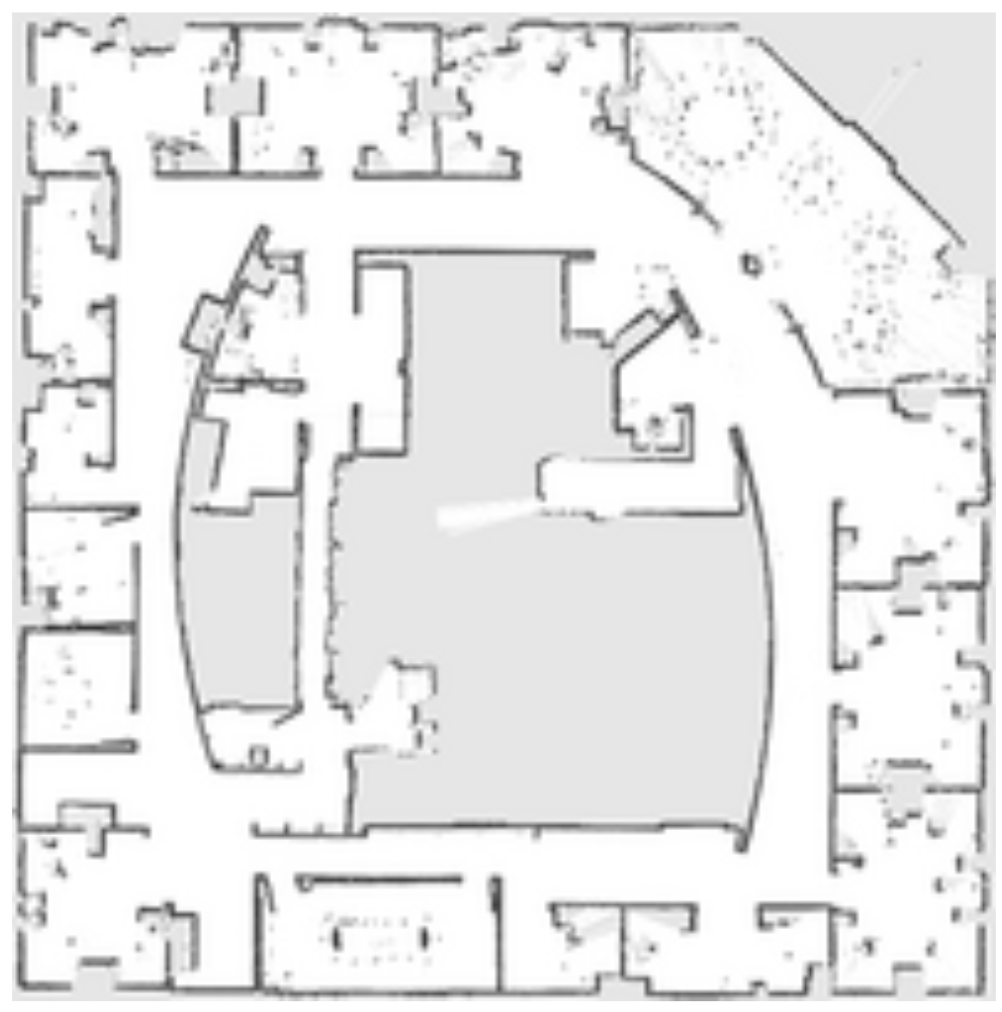
\includegraphics[width=\textwidth]{../images/IntelResearchLab_GroundTruth.png}
        \caption{Actual Intel Research Lab.}
        \label{fig:intel_ground_truth}
    \end{subfigure}
    \hspace{0.3in}
    \begin{subfigure}[t]{0.32\textwidth}
        \centering
        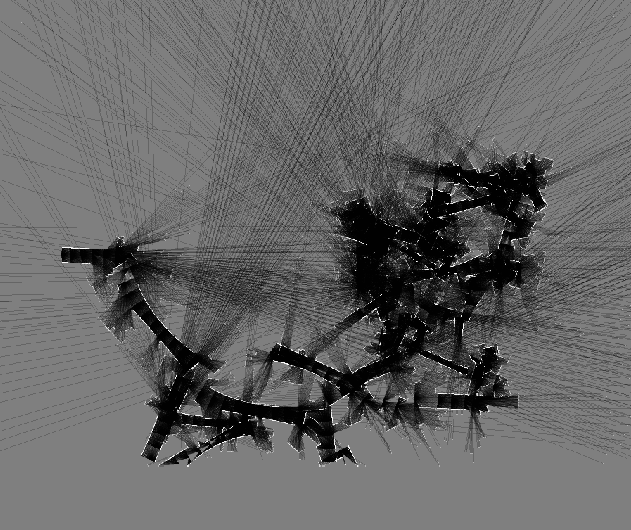
\includegraphics[width=\textwidth]{../images/IntelResearchLab_output.png}
        \caption{Output of SLAM system.}
        \label{fig:intel_occ_grid}
    \end{subfigure}
    \caption{Ground truth vs. SLAM output on the Intel Research Lab dataset.}
    \label{fig:intel_gt_vs_output}
\end{figure}

Production-scale SLAM systems span entire fields of research and take teams of researchers years to
implement and refine.
The results of this project are therefore a commendable achievement given the time constraints,
lack of prior experience, and available resources.

\section{Future Work}

Several directions could improve the system:

\begin{itemize}
    \item \textbf{Point-to-plane correspondence matching.}
          Minimizing the distance from a source point to the plane containing its corresponding target
          point is more robust to noise than point-to-point matching, particularly in planar
          environments. 

    \item \textbf{Sensor fusion with an Extended Kalman Filter.}
          An EKF could intelligently weight contributions from odometry and lidar, especially during
          rotations where ICP alone performs poorly.

    \item \textbf{Scaling to larger environments.}
          All parameters and data structures are tuned for a small, controlled arena.
          Adapting to larger maps would require algorithmic improvements to loop closure candidate
          search, correspondence matching, and optimization.
\end{itemize}

% ============================================================
%  REFERENCES
% ============================================================
\chapter*{References}
\addcontentsline{toc}{chapter}{References}

% TODO: populate references before submission.
\vspace{1cm}
\noindent\textit{References to be added.}

% ============================================================
%  APPENDIX
% ============================================================
\appendix

\chapter{Representative Source Code}
\label{app:code}

Source code for this project is submitted in electronic format alongside this report.
The source code can be found at \href{}{Github Repository}

\vspace{1cm}
\noindent\textit{Code snippets to be added.}

\end{document}
